\clearemptydoublepage
\chapter{Contribution : OCL CSP}
In this chapter we'll cover the bulk of the CSPs which model OCL operations.
Because of our use of a dummy variable in our encoding of collections, the CSPs will often have to model the semantics of the OCL operations around them.
\ytodo{This can, in most cases, also manage the behaviour of invalid or void expressions.}

\begin{figure}[!ht]
    \centering
    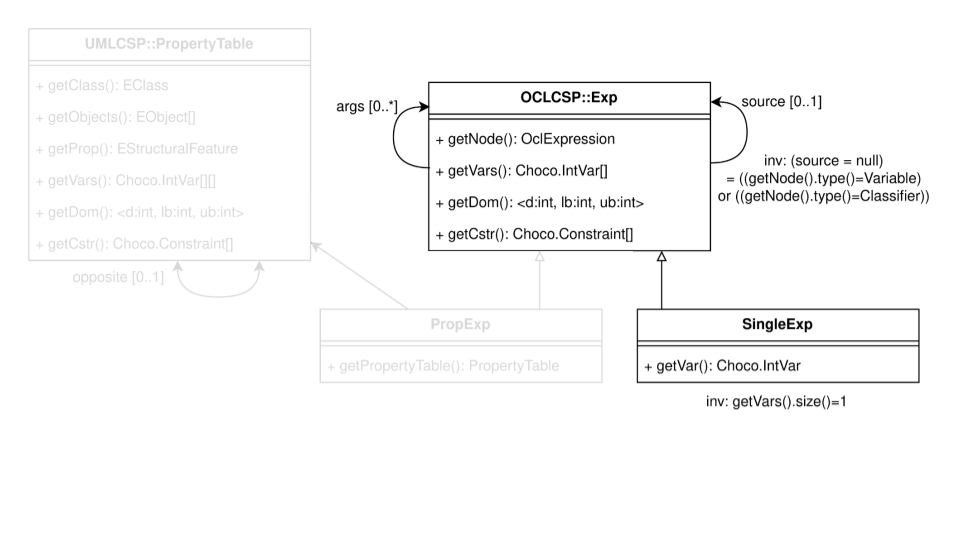
\includegraphics[trim={0 0 0 0},width=1\linewidth]{Contributions/OCLCSP/figures/OCLCSPMM.png}
    \caption{metamodel of expressions in OCLCSP}
    \label{fig:mm:oclcsp}
\end{figure}
Using our \textit{map}, are now on the side of the \textit{OCL CSP}, for which all models inherit from \inlineocl{Exp}, which corresponds to a \inlineocl{OclExpression}.
Every OCL expression will be associated to a CSP: a collection of variables holding the result of the operation, their initial shared domain, and constraints modeling the semantics of the operation.
OCL expressions generally have a \textit{source}, and can have \textit{arguments}, all of which are also OCL expressions (the source can be understood as a special argument).
When building a CSP, we may use information found in the arguments to determine the number of variables required, and their domain.
% All models will have access to information specified here, such as details about domain ranges for intermediate variables.
We've added the special case of \inlineocl{Singleton} which will be used for arithmetic, relational and logic operations, and some other operations operations such as \inlineocl{sum} and \inlineocl{first}.

\begin{figure}[!ht]
    \centering
    \begin{subfigure}[t]{0.48\linewidth}
        \centering
        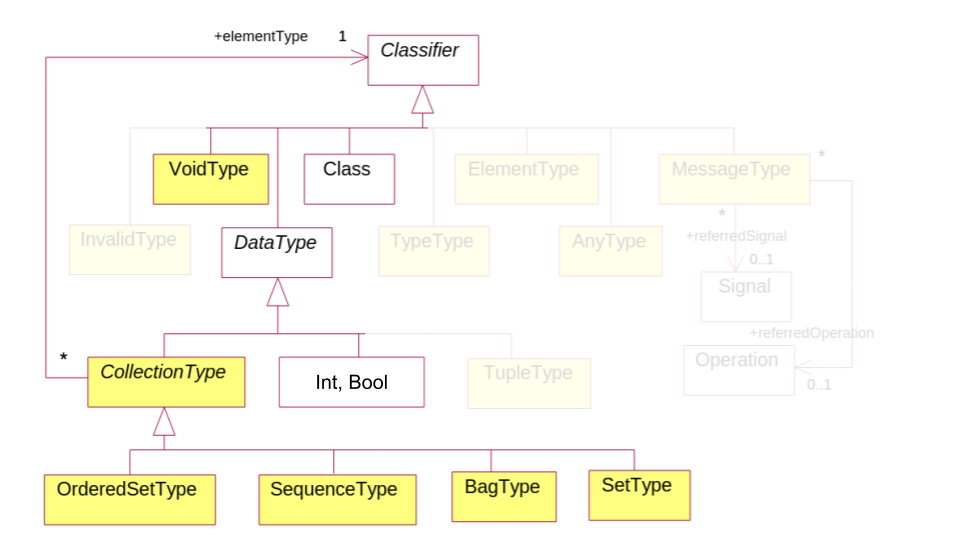
\includegraphics[trim={0 0 0 0},width=1\linewidth]{Contributions/OCLCSP/figures/ocltypecoverage.png}
        \caption{OCL Type Coverage}
    \end{subfigure}
    \hfill
    \begin{subfigure}[t]{0.48\linewidth}
        \centering
        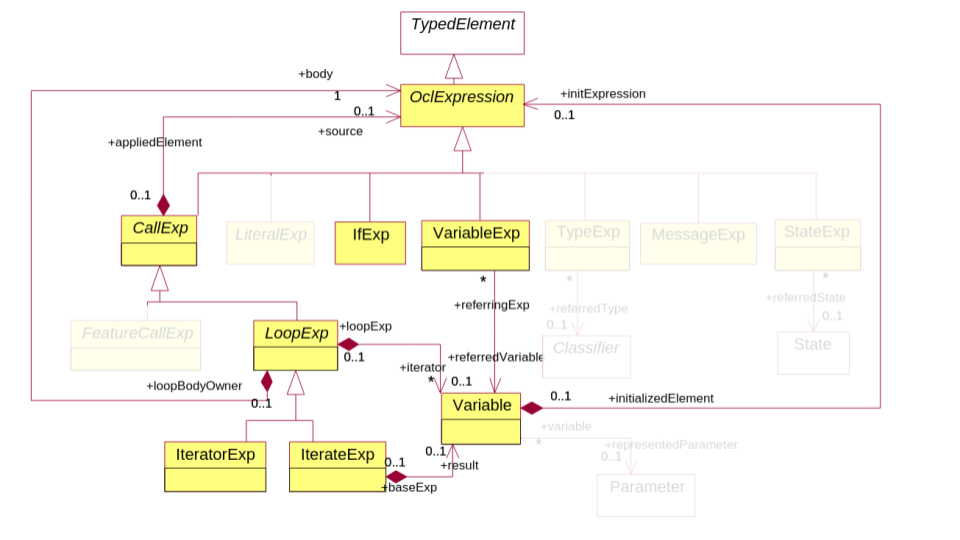
\includegraphics[trim={0 0 0 0},width=1\linewidth]{Contributions/OCLCSP/figures/oclexpressionMMcoverage.png}
        \caption{OCL Expression MMCoverage}
    \end{subfigure}
\end{figure}
In this chapter we'll cover most of this subset of OCL.
For types this means focusing on Collections of booleans, integers and Objects (references).
For the OCL expression metamodel, we cover most CallExp on collections of booleans, integers and Objects.


\begin{table}[!ht]
    \begin{tabular}{|l|l|l|l|l|l|l|}
    \hline
    src \textbackslash out       & bool                                                                                                                            & int                                                                                            & element                                                                    & collection                                                                                        & Sequence                                                                            & Bag                                                                                  \\ \hline
    bool                         & \cellcolor[HTML]{9AFF99}and                                                                                                     &                                                                                                &                                                                            &                                                                                                   &                                                                                     &                                                                                      \\ \hline
    int                          & \cellcolor[HTML]{9AFF99}\textless{}                                                                                             & \cellcolor[HTML]{9AFF99}+                                                                      &                                                                            &                                                                                                   &                                                                                     &                                                                                      \\ \hline
                                 & \cellcolor[HTML]{DAE8FC}                                                                                                        & \cellcolor[HTML]{CBCEFB}                                                                       & \cellcolor[HTML]{9698ED}                                                   & \cellcolor[HTML]{9698ED}                                                                          & \cellcolor[HTML]{96FFFB}asSequence                                                  & \cellcolor[HTML]{96FFFB}                                                             \\ \cline{6-6}
    \multirow{-2}{*}{collection} & \multirow{-2}{*}{\cellcolor[HTML]{DAE8FC}\begin{tabular}[c]{@{}l@{}}=, \textless{}\textgreater\\ includes, forall\end{tabular}} & \multirow{-2}{*}{\cellcolor[HTML]{CBCEFB}\begin{tabular}[c]{@{}l@{}}size\\ count\end{tabular}} & \multirow{-2}{*}{\cellcolor[HTML]{9698ED}any}                              & \multirow{-2}{*}{\cellcolor[HTML]{9698ED}\begin{tabular}[c]{@{}l@{}}select\\ reject\end{tabular}} & \cellcolor[HTML]{9698ED}sortedBy                                                    & \multirow{-2}{*}{\cellcolor[HTML]{96FFFB}asBag}                                      \\ \hline
    Sequence                     &                                                                                                                                 &                                                                                                & \cellcolor[HTML]{FFCCC9}\begin{tabular}[c]{@{}l@{}}first\\ at\end{tabular} &                                                                                                   & \cellcolor[HTML]{FFCCC9}\begin{tabular}[c]{@{}l@{}}subSequence\\ union\end{tabular} &                                                                                      \\ \hline
    Bag                          &                                                                                                                                 &                                                                                                &                                                                            &                                                                                                   &                                                                                     & \cellcolor[HTML]{FFFC9E}\begin{tabular}[c]{@{}l@{}}union\\ intersection\end{tabular} \\ \hline
    \end{tabular}
\end{table}
With this table we want to describe how we have divided the different operations across different sections.
For the following sections we'll be grouping operations based on input amd output type: in green we have grouped operation for which the input and output are integers or booleans, and of type \inlineocl{Singleton}.
For collections, in various shades of blue, we'll split based on output: \inlineocl{Singleton} integer, \inlineocl{Singleton} boolean, elements and collections, and typed collections.
For typed collections, the split is on whether the collection is ordered, in red, or not, in yellow.
\begin{figure}[!ht]
    \centering
    \includegraphics[trim={0 0 0 0},width=1\linewidth]{Contributions/OCLCSP/figures/cheatsheetcoverage.png}
    \caption{cheat sheet coverage in OCLCSP}
    \label{fig:mm:oclcsp}
\end{figure}
We can similarly color the OCL cheat sheet, and show our coverage with a bit more detail.
We can see the previous chapter on OCL navigation in pink.
We can also clearly see operations we don't cover.
Not present in the following sections are \inlineocl{collect} and \inlineocl{iterate}, though some special cases are employed in the models of collection operations, such as \inlineocl{select} and \inlineocl{forall}.
Other operations which aren't included but can be inferred, such as: \inlineocl{allInstances} and other typed based operations.
A similar encoding could also provide coverage for \textit{non-flat} collections and their associated operations, enumerations and tuples.
Not covered with our method are operations on real numbers, and strings.

The first section covers integer and boolean operations.
Collection operations are split across result types: operations of section 2 result in integer, section 3 in booleans, section 4 in collections.
Collection type casting operations are in section 5, and typed collection operations are found in the following sections. 
The type casting operation are among some of the more complicated ones, but most are much less complex, and some are even simple.

\subsection*{..metamodel of the CSPs?}

All of the following CSP will have the same pattern as for the navigation CSP.
\begin{equation}\label{csp:operationGC}
    operation(X,y):
    \begin{cases}
        GlobalConstraint1(X,X')\\
        GlobalConstraint2(X',y)
    \end{cases}
\end{equation}
Where the operation is described as a conjunction of global constraints.
We will use uppercase letters such as $X$ to indicate arrays of variables.
We will use lowercase letters, here $y$ to indicate a single variables.
We will also generally use X for \textit{source} variables, and Y for the variables encoding the result of an operation.
Commonly we'll need to introduce intermediate variables, such as $X'$.
Importantly regarding propagation, for all these CSP: if the input variables $X$ are solved, their domains have only one value, the output variables $Y$ is also solved.

Some times we will have to predicate on individual variables of the arrays.
\begin{equation}\label{csp:operationI}
    operation(X,Y):
    \begin{cases}
        \forall i \in [1..|X|]\\
        ~~ y_i = x_i \times 3
    \end{cases}
\end{equation}
Here each variable is $Y$ is equal to its corresponding value in $X$ times three.
Some of the operation will also take the result of an expression, which in most cases doesn't apply to the source variables $X$.
\begin{equation}\label{csp:operationEXP}
    operation(X,y,exp):
    \begin{cases}
        y = \llbracket exp(X)\rrbracket
    \end{cases}
\end{equation}
In this example, $y$ is equal to the result of applying $exp$ on $X$.
This appears is only a few cases, such as \inlineocl{forall} and \inlineocl{select}
Here we also introduce the $\llbracket \rrbracket$ notation indicating we're interpreting a boolean as an integer.

\newpage
\subsubsection*{Example in Java Code}
\begin{lstlisting}
class SumCSP extends ExpCSP implements Singleton {
    IntVar sum;
    //int d,ub,lb;

    public SumCSP(CSP csp, Exp src){
        super(csp,src);
        //src.vars() is X
        //this.var() is y
        IntVar nullcount = csp.model().count("", src.null(), src.vars());
        IntVar nullsum = src.null().mul(nullcount).intVar();
        IntVar rawsum = csp.model().sum("", src.vars());
        sum = rawsum.sub(nullsum).intVar();
    }

    //Singleton methods
    public IntVar var() {return sum;}
}
\end{lstlisting}
Here we can see how an operation is translated into Java using the Choco API in our OCLinChoco project. In this code \inlineocl{csp.model()} is a Choco model, and IntVar is imported from Choco. 
This model is further explained in its section, but we already see how it matches the same pattern, and explicitly how we access information when building the CSPs.
The overall CSP is given to each Object representing a node of an OCL AST applied to an instance (collection of Objects), for them to each add their variables and constraints.
Intermediate variables are generally instantiated by applying a global constraint, but we also can access a lot of information from the source object.

\newpage
\section{CP Models for OCL Integer and Boolean Operations}
While in many cases modeling OCL arithmetic and logic on attributes is straight forward, there are edge cases we must consider.
The reason for this is UML allowing for optional properties: \inlineocl{[0..1] Boolean} and \inlineocl{[0..1] Int}.
For situations where the property is required, we can simply use arithmetic and logic operations.

\subsection{3-valued logic for OCL}
OCL is fundamentally a 4-valued logic, with values: true, false, void, and invalid.
Both Void and invalid behave similarly for the logical operations, and we have chosen to combine them in our encoding.
However invalid expressions can often be statically detected, and stop the interpretation before building the CSP.
OCL\# also collapses OCL to a 3-valued logic using the empty set $\emptyset$ to encode void and invalid expressions. \ytodo{because RFOL}

\begin{table}[!ht]
    \begin{tabular}{c|c|c|c|c|c|c}
    a & b & a and b & a or b & a xor b & a implies b & not a \\ \hline
    2 & 2 & 2       & 2      & 0       & 2           & 0     \\ \hline
    2 & 1 & 1       & 2      & 1       & 1           & 0     \\ \hline
    2 & 0 & 0       & 2      & 2       & 0           & 0     \\ \hline
    1 & 2 & 1       & 2      & 1       & 2           & 1     \\ \hline
    1 & 1 & 1       & 1      & 1       & 1           & 1     \\ \hline
    1 & 0 & 0       & 1      & 1       & 1           & 1     \\ \hline
    0 & 2 & 0       & 2      & 2       & 2           & 2     \\ \hline
    0 & 1 & 0       & 1      & 1       & 1           & 2     \\ \hline
    0 & 0 & 0       & 0      & 0       & 2           & 2     
    \end{tabular}
\end{table}
In this table we find the semantics for boolean operations in OCL, combining both invalid and void into \textit{maybe}.
For this table we have chosen $\top$=2, \textit{maybe}=1 $\bot$=0.
The semantics for these logical operations encoded with integers can be simply modeled with integer operations:
\begin{itemize}
    \item $\neg a \equiv 2-a$
    \item $a \wedge b \equiv min(a,b)$
    \item $a \vee b \equiv max(a,b)$
    \item $a \rightarrow b \equiv max(2-a,b)$
    \item $a \oplus b \equiv min(2-min(a,b),max(a,b))$
\end{itemize}
We can see these models employ $min$ and $max$ as $and$ and $or$, and $\top -x$ for not, and model \textit{implication} and \textit{the exclusive or} on top:
\begin{itemize}
    \item $a \rightarrow b \equiv (\neg a \vee b)$
    \item $a \oplus b \equiv (\neg(a \wedge b) \wedge (a \vee b))$
\end{itemize}

\subsection{Property encoding to 3-valued logic for optional Booleans}
\begin{figure}[!ht]
    \centering
    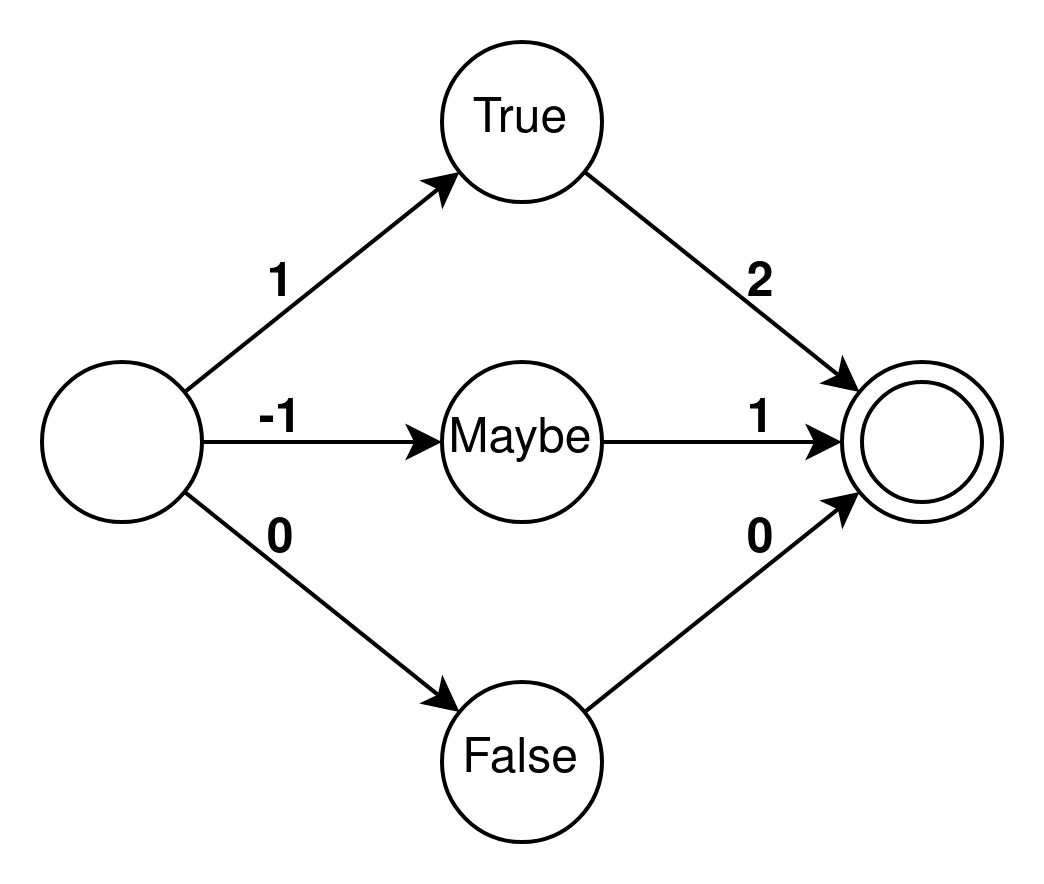
\includegraphics[trim={0 30 0 0},width=0.5\linewidth]{Contributions/OCLCSP/Operations/figures/negbool2halfboolAFD.png}
    \caption{Part of the tree for \inlineocl{src.forall(a,b,c| (a<b and b<c) implies (a+b=c+c))}}
    \label{fig:forallexample}
\end{figure}
In our base encoding for properties, True equals 1, False equals 0, and no information is -1.
We could implement a different encoding for booleans, or simply convert from one encoding to the other using an regular expression constraint based on the AFD here.

\subsection{Operations with Optional Integers}
In the OCL Specification: \textit{The interpretation of operations is considered strict [...]. Hence, an
invalid or null argument value causes an invalid operation result. This ensures the propagation of error conditions.}
This means expressions such as \inlineocl{2 + null} are \textit{invalid}, and generally invalidate the whole model.


To follow the specification and and only handle valid OCL, we can fail by making adding a contradiction to the constraint model, essentially adding \texit{AND False} appropriately.

Taking addition as an example: $x+y=z$, becomes $x+y=z \wedge x \neq d \wedge y \neq d$, to fail because invalid expression: 2 + d = False. In this case: models with data and solver configurations forcing an absence will be invalid and the will be no solution to the CSP, otherwise it will populate all the attributes with values.

However, we can also relax the arithmetic. 
If we didn't want to force the presence of attributes or fail, and wanted to maybe ignore operations on absent values, we can exchange the d value of a variable with another.
For instance $x+y=z$, becomes $$x'+y'=z \wedge (x=d => x'=0) \wedge (x \neq d => x'=x) \wedge (y=d => y'=0) \wedge (y \neq d => y'=y)$$
Here, if either $x$ or $y$ are null, we replace their value with 0 in $x'$ and $y'$, skipping the addition.
We could always interpret null as 0, or choose an interpretation which skips the operations, such as 1 in multiplication, \textit{infinity} in \textit{less than}, etc.. 
% Summing over collection similarly 

\ytodo{OCL\# : in OCL- there is no invalid or null, and arithmetic isn't done with missing values? Check this.}

\newpage
\section{CP Models for OCL Collection to Int Operations}
In this section we'll consider expressions of the type \inlineocl{src.op()} where \inlineocl{src} is a collection and the result of the operation is a single integer.


\subsection{size()}
Consider the expression \inlineocl{src.size()}, where \inlineocl{src} is an expression resulting in a collection: the \inlineocl{size} operation returns the size of the \inlineocl{src} collection.

Because of our encoding with collections using dummy variables, we define the size constraint around them, where $X$ are the variables representing \inlineocl{src} and $y$ is the output of the \inlineocl{size} operation: 
\begin{equation}\label{def:size}
    size(X,y) \iff y = \sum_{0 < i \leq |X|} \llbracket x_i \neq d \rrbracket
\end{equation}
This definition states that $y$ is equal to the count of values not equal to $d$.
Reformulation using Global Constraints:
\begin{equation}\label{csp:size}
    size(X,y):
    \begin{cases}
        count(d,X,y') \\
        y = |X|-y'
    \end{cases}
\end{equation}
In this model, we simply count the number of times the dummy value $d$ appears in the source collection $X$.
The output $y$ is constrained to equal the difference between the size of the variable array $X$, and the count of $d$: $y = |X|-y'$.

For example, given the collection $[3,1,2,d,d]$ we count 2 $d$, the size of the array is 5, so the number of values in the collection is 5-2=3. 

\subsection{sum()}
Consider the expression \inlineocl{src.sum()}, where \inlineocl{src} is an expression resulting in a collection of integers: the \inlineocl{sum} operation returns the sum of the \inlineocl{src} collection.

Because of our encoding with collections using dummy variables, we define the sum constraint around them, where $X$ are the variables representing \inlineocl{src} and $y$ is the output of the \inlineocl{sum} operation.
The sum operation can be defined similarly to \inlineocl{size}, by additionally multiplying by the value of each variable of the source:  
% Definition:
\begin{equation}\label{def:sum}
    sum(X,y) \iff y = \sum_{0 < i \leq |X|} x_i * \llbracket x_i \neq d \rrbracket
\end{equation}
This definition states that $y$ is equal to the sum of values not equal to $d$.
Among the globals there is a sum constraint which we can employ.
Reformulation using Global Constraints:
\begin{equation}\label{csp:sum}
    sum(X,y):
    \begin{cases}
        count(d,X,s') \\
        y = sum(X) - ds'
    \end{cases}
\end{equation}
In this model use $y=sum(X)$, and then simply subtracts the dummies.

For example, given the collection $[3,1,2,d,d]$ we count 2 $d$.
The sum of the array being $6+2d$, we use the count to negate the occurrences of $d$:
$6+2d-2d$.

\subsection{count(e)}
Consider the expression \inlineocl{src.count(e)}, where \inlineocl{src} is an expression resulting in a collection and \inlineocl{e} is an expression resulting in a single element: the \inlineocl{count} operation returns the count of \inlineocl{e} in \inlineocl{src}.
With $X$ as the variables representing \inlineocl{src}, $y$ as the variable representing \inlineocl{e}, and $z$ representing the count, we can define the operation as follows:
\begin{equation}\label{def:count}
    count(X,y,z) \iff z = \sum_{0 < i \leq |X|} \llbracket x_i = y \rrbracket
\end{equation}
Meaning simply applying the appropriate global:
\begin{equation}\label{csp:count}
    count(X,y,z):
    \begin{cases}
        count(y,X,z)
    \end{cases}
\end{equation}

\subsection{max()}
Consider the expression \inlineocl{src.max()}, where \inlineocl{src} is an expression resulting in a collection of integers: the \inlineocl{max} operation returns the highest value in the \inlineocl{src} collection:
\begin{equation}\label{def:max}
    max(X,y) \iff (\forall x \in X, y \geq x) \wedge (\exists x \in X, x=y) 
\end{equation}
Reformulation using Global Constraints:
\begin{equation}\label{csp:max}
    max(X,y):
    \begin{cases}
        maximum(y,X)
    \end{cases}
\end{equation}
Because for our encoding using the minimum of the domain as the dummy it doesn't effect the constraint model.

\subsection{min()}
Consider the expression \inlineocl{src.min()}, where \inlineocl{src} is an expression resulting in a collection of integers: the \inlineocl{min} operation returns the lowest value in the \inlineocl{src} collection.

Because of our encoding with collections using dummy variables, and using the lowest value of the domain as dummy value, our definition of minimum needs to exclude that value:
\begin{equation}\label{def:min}
    min(X,y) \iff \\
    ~~(\forall x \in X, x\neq d \iff y \leq x)\\
    ~\wedge (\exists x \in X, x=y)\\
    ~\wedge y\neq d
\end{equation}
In order to employ the $minimum$ global constraint, we create a copy of the list, where variables equal to $d$ get flipped to the beyond the upper bound of the domain, giving us the following reformulation using Global Constraints:
\begin{equation}\label{csp:min}
    min(X,y):
    \begin{cases}
        \forall i \in [1..z]\\
        ~~x'_i = x_i - (2d+1)*\llbracket x_i=d \rrbracket \\
        minimum(y,X')
    \end{cases}
\end{equation}
For example, given the collection $[3,1,2,d,d]$ we create the copy flipping the dummy: $[3,1,2,-2d+1,-2d+1]$, because $d$ is the smallest value of the domain and $-2d+1$ is just above the domain of valid values in our encoding.

\newpage
\section{CP Models for OCL Collection to Bool Operations}
\input{Contributions/OCLCSP/Operations/collection2bool}

\newpage
\section{CP Models for OCL Collection Operations}
In this section we cover the operations which take collections and return collections.
% \subsection{operation()}
% Consider the expression \inlineocl{src.operation()}, where 
% Formal Definition:
% \begin{equation}\label{def:operation}
%     operation(X,y) \iff \llbracket x_i \neq d \rrbracket
% \end{equation}

% Reformulation using Global Constraints:
% \begin{equation}\label{csp:operation}
%     operation(X,y):
%     \begin{cases}

%     \end{cases}
% \end{equation}
% \newpage
\subsection{select(exp)}
Consider the expression \inlineocl{src.select(exp)}, where \inlineocl{src} is an expression resulting in a collection and \inlineocl{exp} is a predicate: the output of the operation is the sub-collection of elements for which the predicate is true.
This operation can have at most one iterator variable.
% Formal Definition:
% \begin{equation}\label{def:select}
%     select(X,Y,exp) \iff
% \end{equation}

% Reformulation using Global Constraints:
\begin{equation}\label{csp:select}
    select(X,Y,exp):
    \begin{cases}
        y_i = d - (d-x_i)*\llbracket exp(x_i) \rrbracket
    \end{cases}
\end{equation}
For this model we first assume the value is filtered $y_i=d$, then depending on if the expression is true when applied $exp(x_i)$ we add it back the value $x_i$, using $-(d-x_i)$.

% \newpage
\subsection{reject(exp)}
Consider the expression \inlineocl{src.reject(exp)}, where \inlineocl{src} is an expression resulting in a collection of objects or integers and \inlineocl{exp} is a predicate: the output of the operation is the sub-collection of elements for which the predicate is false.
This operation can have at most one iterator variable.
% Formal Definition:
% \begin{equation}\label{def:reject}
%     reject(X,Y,exp) \iff
% \end{equation}

% Reformulation using Global Constraints:
\begin{equation}\label{csp:reject}
    reject(X,Y,exp):
    \begin{cases}
        y_i = d - (d-x_i)*\llbracket \neg exp(x_i) \rrbracket
    \end{cases}
\end{equation}
For this model we first assume the value is filtered $y_i=d$, then depending on if the expression is false when applied $exp(x_i)$ we add it back the value $x_i$, using $-(d-x_i)$.

\newpage
\subsection{any()}
This operation can have at most one iterator variable.
Consider the expression \inlineocl{src.any(exp)}, where \inlineocl{src} is an expression resulting in a collection of objects or integers and \inlineocl{exp} is a predicate: the output of the operation is one of the elements for which the predicate is true.
This operation can have at most one iterator variable.
% Formal Definition:
% \begin{equation}\label{def:any}
%     any(X,Y,exp) \iff
% \end{equation}
% Reformulation using Global Constraints:
\begin{equation}\label{csp:any}
    any(X,y,exp):
    \begin{cases}
        select(X,Y,exp)\\
        asBag(Y,Y')\\
        y = y_1'
    \end{cases}
\end{equation}
For this model, we simply use the selection model to find good values, and use the as bag model to make sure the first value is valid.
Any other way of choosing a valid value could also be chosen.

% \newpage
\subsection{sortedBy(exp)}
This operation can have at most one iterator variable.
Consider the expression \inlineocl{src.sortedBy(exp)}, where \inlineocl{src} is an expression resulting in a collection of objects or integers and \inlineocl{exp} results in an integer: the output of the operation is the sequence of elements with respect to the result of the expression.
% Formal Definition:
% \begin{equation}\label{def:sortedBy}
%     sortedBy(X,Y,exp) \iff
% \end{equation}
Reformulation using Global Constraints:
\begin{equation}\label{csp:sortedBy}
    sortedBy(X,Y,exp):
    \begin{cases}
        stable\_keysort(\langle K,X\rangle,\langle K',Y\rangle,1) \\
        ~~k_i=exp(x_i), \forall i \in [1,z]
        % ~~k'_i=\llbracket y_i=d \rrbracket, \forall i \in [1,z]
    \end{cases}
\end{equation}
For this we simply apply the key sort global constraint, using the result of the expression as key.

% \subsection{collect()}
% Consider the expression \inlineocl{src.collect(exp)}, where exp is an expression.
% Formal Definition:
% \begin{equation}\label{def:collect}
%     collect(X,Y,exp) \iff
% \end{equation}

% Reformulation using Global Constraints:
% \begin{equation}\label{csp:collect}
%     collect(X,Y,exp):
%     \begin{cases}
%         y_i = d - (d-x_i)*\llbracket not exp(x_i) \rrbracket
%     \end{cases}
% \end{equation}

\newpage
\section{CP Models for OCL Collection Type Casting Operations}
\input{Contributions/OCLCSP/Operations/typecasting}

\newpage
\section{CP Models for OCL Sequence and Ordered Set Operations}
\input{Contributions/OCLCSP/Operations/sequence}

\newpage
\section{CP Models for OCL Set and Bag Operations}
In this section we consider operations on unordered collections, namely: bags and sets.

\newpage\subsection{union(exp)}
The models for union between sets, and any other combination of bag and set, are very similar.
For both of these models, we simply append both arrays of variables, and apply the right type casting operation to ensure conformance.

Consider the expression \inlineocl{src.union(exp)}, where \inlineocl{src} is an expression resulting in a set of objects or integers, and \inelineocl(exp) is (an expression resulting in) a set of objects or an integers: the output of the operation is the set equal to the union of \inlineocl{src} and \inlineocl{exp}.
Reformulation using Global Constraints:
\begin{equation}\label{csp:union_setset}
    union\_setset(X,Y,Z):
    \begin{cases}
        X \;\mathbin{\|}\; Y'
        asSet(Y',Y)
    \end{cases}
\end{equation}

Consider the expression \inlineocl{src.union(exp)}, where \inlineocl{src} is an expression resulting in a set or bag of objects or integers, and \inelineocl(exp) is (an expression resulting in) a bag of objects or an integers: the output of the operation is the bag equal to the union of \inlineocl{src} and \inlineocl{exp}.
Reformulation using Global Constraints:
\begin{equation}\label{csp:union_Xbag}
    union\_Xbag(X,Y,Z):
    \begin{cases}
        X \;\mathbin{\|}\; Y'
        asBag(Y',Y)
    \end{cases}
\end{equation}

\newpage\subsection{Intersection}
Consider the expression \inlineocl{src.intersection(exp)}, where \inlineocl{src} is an expression resulting in a set or bag of objects or integers, and \inelineocl(exp) is (an expression resulting in) a set or bag of objects or integers: the output of the operation is the bag equal to the intersection of \inlineocl{src} and \inlineocl{exp}.
Reformulation using Global Constraints:
\begin{equation}\label{csp:intersection}
    intersection(X,Y,Z):
    \begin{cases}
        count(x_i,X,c_i)\\
        count(x_i,Y,c_i')\\
        count(x_i,Z,c_i'')\\
        c_i'' = \llbracket x_i = d \rrbracket * a_i + \llbracket x_i \neq d \rrbracket * min(c_i,c_i')\\
        a_i \geq max(c_i,c_i')\\
        count(z_i,X,b_i)\\
        count(z_i,Y,b_i')\\
        count(z_i,Z,b_i'')\\
        b_i'' = \llbracket z_i = d \rrbracket * a_i' + \llbracket z_i \neq d \rrbracket *min(b,b_i')\\
        a_i' \geq max(b_i,b_i')\\
    \end{cases}
\end{equation}
This model works for all combinations of set and bag, and will result in a set if either argument is a set.
This model can be divided in two similar parts: towards the output, and towards the input.
In the first part, towards the output, we count the occurrences of values of $X$, in $X$ and $Y$, and enforce the count of those values in $Z$ to be the minimum of the two.
In the second part, towards the input, we count the occurrences of values of $Z$, in $X$ and $Y$, and enforce the count of those values in $Z$ to be the minimum of the two.
This second part mainly ensures we don't slip in a value instead of a dummy.
We don't have a count for the exact number of dummies with this model, but we can enforce a lower bound: at least the greatest number of dummies in $X$ and $Y$.

\begin{figure}[!ht]
    \centering
    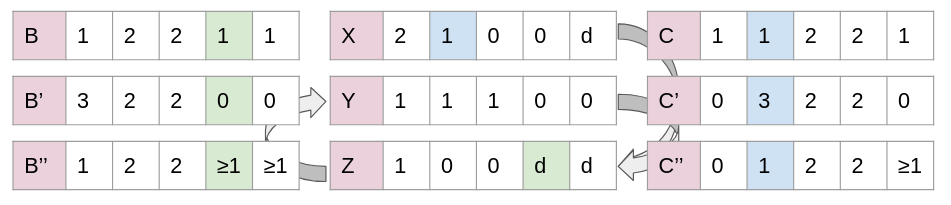
\includegraphics[trim={0 0 0 0},width=1\linewidth]{Contributions/OCLCSP/Operations/figures/intersectCount.png}
    \caption{Visualization of the use of count to model set and bag intersection}
    \label{fig:cumulative}
\end{figure}
In this figure we illustrate a solution and include all the intermediate variables.
In the middle we have $X$, $Y$, and $Z$.
On the right we have the \textit{towards the output} part,
and on the left, the \textit{towards the input} part.
Highlighted in blue we have $x_2$ and its counts in $X$, $Y$, and $Z$.
Highlighted in green we have the mirror with $z_4$ and its counts in $X$, $Y$, and $Z$.

% \begin{equation}\label{csp:intersection_setset}
%     intersection\_setset(X,Y,Z):
%     \begin{cases}
%         b_{i1} = x_i \wedge b_{i2} = 1\\
%         b_{(i+|X|)1} = y_i \wedge b_{i2} = 2\\
%         stable\_keysort(B,B',2)\\
%         c_n \iff (b_{n1}=b_{(n-1)1} \wedge b_{n2}\neq b_{(n-1)2})\\

%     \end{cases}
% \end{equation}

\newpage\subsection{unordered - unordered}
Consider the expression \inlineocl{exp1 - exp2}, where \inlineocl{exp1} is an expression resulting in a set or bag of objects or integers, and \inelineocl{exp2} is (an expression resulting in) a set or bag of objects or an integers: the output of the operation is the set or bag equal to the difference of \inlineocl{exp1} and \inlineocl{exp2}.
The type of the result is the same as \inlineocl{exp1}.
\begin{equation}\label{csp:diff_set}
    diff\_set(X,Y,Z):
    \begin{cases}
        count(x_i,Y,s_i)\\
        b_i \iff (s_i = 0)\\
        z'_i = d - (d-x_i)*\llbracket b_i \rrbracket\\
        sort(Z',\reverse{Z})
    \end{cases}
\end{equation}
This model can be seen as a filter on $X$ for values found in $Y$, and uses a similar model as that for \inlineocl{X.select(x | Y.count(x)=0)}.
And as the OCL describes, this model filters values from $X$ depending on their presence in $Y$, the result of which is in sorted into $Z$.


% \newpage
\subsection{symmetricDifference(exp)}
Consider the expression \inlineocl{src.symmetricDifference(exp)}, where \inlineocl{src} is an expression resulting in a set or bag of objects or integers, and \inelineocl{exp} is (an expression resulting in) a set or bag of objects or an integers: the output of the operation is the set or bag equal to the symmetric difference of \inlineocl{src} and \inlineocl{exp}.
The result of this operation is a set, if both arguments are sets.
\begin{equation}\label{csp:symdiff_set}
    symdiff\_set(X,Y,Z):
    \begin{cases}
        diff\_set(X,Y,S)\\
        diff\_set(Y,X,T)\\
        C = S \;\mathbin{\|}\; T\\
        sort(C,\reverse{Z})
    \end{cases}
\end{equation}
This model simply reuses the model for difference, filtering for both $X$ and $Y$.
The results, $S$ and $T$, are then combined and sorted into the output $Z$.

% \subsection{including}
% \begin{equation}\label{csp:setbagincluding}
%     including\_set(X,Y,Z):
%     \begin{cases}
%         diff\_set(X,Y,S)\\
%         diff\_set(Y,X,T)\\
%         C = S \;\mathbin{\|}\; T\\
%         sort(C,\reverse{Z})
%     \end{cases}
% \end{equation}


% \subsection{excluding}

\newpage
% \section{CP Models for OCL Bag Operations}
% \input{Contributions/OCLCSP/Operations/bag}

\newpage
\section{Experimentation}
\input{Contributions/OCLCSP/Operations/experimentation}

% \section{CP Models for OCL Ordered Set Operations}
% \input{Contributions/OCLCSP/Operations/orderedset}

% \section{CP Models for Class Functions and Global Functions}
% \input{Contributions/OCLCSP/Operations/orderedset}